\documentclass[thesis.tex]{subfiles}
\begin{document}

\chapter{Main}\label{chap:basics}

\section{Overview}
Inspired by Lensing's LightSkin approach~\cite{bib:LightskinPaper}, we want to compute indirect lighting only at specific locations and interpolate the results over multiple pixels, as opposed to techniques like Reflective Shadow Maps or Voxel Cone Tracing \todo{ref related work sections}.
\todo{Advantages/disadvantages}
As in many previous works, we call these locations \emph{Light Caches}.

Our technique consists of three basic steps which are executed in every frame: Cache allocation, indirect lighting and cache interpolation.
The cache allocation pass assigns cells on a regular grid to cache memory, thus creating the caches that are about to be used in this frame.
Using a reflective shadow map, indirect lighting is then computed for all caches.
Finally each pixel interpolates an indirect lighting value using all neighboring caches within the grid.

Each of the following major sections will explain one of these stages and their interdependencies.
The last major section of this chapter will elaborate several implementation details, some of them crucial to the overall performance.\\
Many parts of our approach are based on several well-known techniques of which most have already been discussed in \autoref{chap:prevwork} and \autoref{chap:basics}.
Where necessary, details of the respective algorithms will be elaborated to address specifics implied by the overall technique.

\section{Cache Allocation}
Since the goal of this work is a fully dynamic solution that works without any pre-computations, it is necessary to place all caches at runtime, as opposed to LightSkin~\cite{bib:LightskinPaper} where caches are placed in a computational intense preprocessing step.
Before we introduce our solution, several general implications of such an approach are elaborated.

\subsection{General Properties and Requirements of Dynamic Cache Placement}
Compared to a precomputation based approach, there are several intrinsic advantages which can be expected of a dynamic light cache placement.
Since we target for a single bounce of indirect light, caches are only used by locations that lie in the current view frustum (for multiple bounces however, it might be necessary to transfer lights between caches).
Also it should be possible to decrease the number of caches for distant objects, thus keeping screen-space cache density within a given bound.
Both properties result in a much lower memory footprint especially for large scenes.

While it can be very beneficial to place caches dependent on the current view, this also may introduce several temporal artifacts if caches disappear or move, i.e. strong changes in indirect lighting from one frame to the next.
Additionally, it is necessary to guarantee that target pixels have easy access to a certain number of caches to be able to interpolate them.
Note that the interpolation pass can have temporal coherence problems on its own, as the assignment of a cache to its surrounding world positions needs to be stable, no matter how densely they are sampled, i.e. how many pixels a given world space area covers.

So far, the data requirements of each cache have not been defined yet.
Precomputed caches can naturally hold almost arbitrary data (as long as a given memory bound is not exceeded).
Dynamic caches on the other hand need to acquire their data every frame, which is not only costly performance-wise but may also cancel out certain types of data as it may not be accessible. For example LightSkin~\cite{bib:LightskinPaper} needs to a rather complex area metric for each cache that can not be computed in real-time.
Naturally, such constraints also affect the following lighting and interpolation stages tremendously.

We evaluated several approaches before we came up with our final algorithm.
If you are interested you can read the summary of these attempts in \autoref{chap:abandoned}.

\subsection{Cascaded Cache Address Volume}
To cancel out temporal artifacts entirely, we decided to place caches only at the nodes of a regular world space grid.
The main disadvantage of this method is, that caches are not placed on surfaces and thus can not have a specific orientation.\\
Since only a small fraction of all grid cells contains any caches, they are stored in a separate buffer and only their addresses are saved within the grid.
Accordingly, we call this grid the \emph{Cache Address Volume (CAV)}.
This approach reduces not only the memory consumption drastically, it makes it also much easier to perform the lighting for each cache, as they lie now consecutive in memory instead of being scattered within a volume.

During the cache allocation pass the CAV is cleared and then refilled depending on the current view.
This is done by a full-screen pass, using the per-pixel world-positions from the previously rendered scene (which can be acquired using the depth buffer).
Each pixel allocates caches at the eight nearest CAV cells.
If an affected cell already contains a valid cache address, it is skipped as pixels do not introduce any data besides the cache allocation itself.
Since neighboring pixels often access the same grid cells, there is room for some optimizations using shared memory which are explained in \autoref{sec:impl:cachealloc}.

\subsubsection{Cascading}
Similar to Cascaded Light Propagation Volumes~\cite{bib:lpt} a set of nested CAV cascades are centered around the camera.
This introduces a distance dependent level of detail and keeps the number of caches constant, even for large scenes.
The cascade positions are snapped to multiples of their grid size to ensure consistent lighting results. \todo{elaborate the snapping-whys further?}
For simplicity, all CAV cascades are cubes of the same resolution with their grid size doubling for each consecutive cascade.

Caches are only allocated using the smallest CAV cascade which encloses a given pixel world-position.
Since a pixel needs to be able to access eight different neighboring cells, decision boundaries are used which are smaller than the actual extent of the cascade.
As the snapped movement introduces temporal incoherency, we move the decision boundaries smoothly with the camera and shrink them further by another grid cell size to ensure that the decision boundaries are fully enclosed in their respective cascades.

Additionally, there are transition areas between two successive cascades.
A transition area is as wide as the grid cell size of the smaller involved cascade.
Within these areas, caches are allocated in both cascades to make it possible to avoid hard edges during the interpolation stage late on.\\

Contrary to Light Propagation Volumes, the cascades are not displaced with the view direction, but strictly centered around the camera position as this helps to keep the level of detail stable against view rotations.\\
While this means that a very large portion of each cascade is never used at all, the costs are still rather low since there are no computations involved for empty cells.
Also, the memory footprint is small: %nevertheless
A high detailed setup consists of four cascades, each with a resolution of $64^3$.
With four byte address in each cell, this results in 4MB for all CAV cascades.
\todo{image showing cascades!}

\section{Indirect Lighting}
The indirect lighting of the caches relies on reflective shadow maps (see \todo{citation needed}).
In principle each cache iterates on the entire RSM to retrieve the encoded lighting informations.
The following chapters explain how this information is processed and how the results are saved for later interpolation.

\subsection{Diffuse Lighting}
We make use of the common separation of diffuse and specular lighting, making the later an optional feature that may be deactivated to save resources if necessary. \todo{principle should be in the basics chapter}
Diffuse lighting is comparatively easy to compute and represent since, for a given position and reflectivity, it is a low frequency function over a surface normal, independently of the view direction.

Recall the rendering equation for pure diffuse surfaces:
\begin{equation}
L_o (\mathrm{x}) = \frac{\rho}{\pi}\int\limits_{2\pi sr} L_i(x,\omega_i) \cdot \cos\theta \,\mathrm{d}\omega_i
\end{equation}
Using the reflective shadow map, an approximation of the integral can be expressed as a sum over $n$ virtual area lights:
\begin{align}
L_o (\mathrm{x})
&=\frac{\rho}{\pi}\sum\limits_{i=0}^{n} L_i \cdot (\hat{\mathbf{n}} \cdot \hat{\mathbf{d}}_i)^+ = \\
&=\frac{\rho}{\pi}\sum\limits_{i=0}^{n} \frac{I_i }{||\mathrm{x} - \mathrm{x}_i||^2 +  A_i} \cdot (\hat{\mathbf{n}} \cdot \hat{\mathbf{d}}_i)^+ \\
&=\frac{\rho}{\pi}\sum\limits_{i=0}^{n} \frac{\frac{\phi_i}{\pi} (\hat{\mathbf{n}}_i \cdot (-\hat{\mathbf{d}}_i) )^+}{||\mathrm{x} - \mathrm{x}_i||^2 +  A_i} \cdot (\hat{\mathbf{n}} \cdot \hat{\mathbf{d}}_i)^+
\end{align}
\todo{Where do we explain the disc light thing? Need to derive this formular much slower!}
%Each RSM pixel is interpreted as a disc-shaped light as described by Lensing (see \todo{either explain here or earlier}).

The reflectivity $\rho$ is usually given by a texture and varies per pixel.
However, since it is not part of the sum over all RSM pixels, it can be applied easily during the cache interpolation stage.\\
As caches are not placed on surfaces, there is no known normal vector $\hat{\mathbf{n}}$.
The only other quantity that does not depend on the RSM is the position, which is known for each cache.
Accordingly, each cache saves irradiance as a function over the normal vector.
We chose a low-order spherical harmonics representation since it allows iterative computation and easy evaluation at runtime.\\ 
The irradiance contribution of a single light to the spherical harmonics coefficients can be derived analytically. \todo{put the meat of all this in prerequisites}
For a single light, the irradiance is symmetric to its direction.
Using this property, rotated Zonal Harmonic coefficients can provide an much easier way of deriving the irradiance contribution than directly using Spherical Harmonics.
First, Zonal Harmonic coefficients $z_l$ are computed for a fixed light direction, pointing to $(0,0,1)$.
\begin{align}
z_l =&\int\limits_{2 \pi sr} L_i \cdot (\omega \cdot (0,0,1))^+ \cdot y^0_l(\omega) \,\mathrm{d}\omega\\
=&\int\limits_{2 \pi sr} L_i \cdot \cos\theta \cdot y^0_l(\omega) \,\mathrm{d}\omega
\end{align}
Note that by integrating only over the upper hemisphere, the cosine does not need to be explicitly clamped.
Due to the rotation invariance of Spherical Harmonics, the resulting Zonal Harmonics coefficients can be rotated to the light direction $\hat{\mathbf{d}}_i$.
\begin{equation} \label{eq:zonalrotate}
	c_l^m = \sqrt{\frac{4\pi}{2l+1}} \cdot z_l \cdot y_l^m(\hat{\mathbf{d}}_i)
\end{equation}
The resulting expressions for the first three SH bands can be found in \autoref{chap:shcosinelobe}.

To perform the diffuse cache lighting, the coefficients for all virtual lights are accumulated and saved into the cache buffer for later evaluation. \todo{add a note on how many bandy are required}

\subsection{Specular Lighting}
optional...

\subsection{Indirect Shadows}
optional but crucial, difficult .... ....


\subsubsection{Scene Voxelization}

\subsubsection{Cone Casts on Filtered Reflective Shadow Maps}


\section{Cache Interpolation}



\section{Implementation}

\emph{As many as possible details should be delayed into this chapter. If it gets large or starts to mirror the main part, make it a chapter!}

This is the right place for describing how to use Compute, OpenGL etc. for achieving the rather abstract formulated goals of the sections before.

Deferred Renderer, 32bits per Layer RGB(A) srgb - Diffuse, RG 16snorm - Normals with angles, extra infos todo, R32F Depth Buffer (swapped near/far)\\
(This detail belongs more or less to Eva...)

\subsection{Pipeline Overview}

\begin{figure}[h]
	\centering
	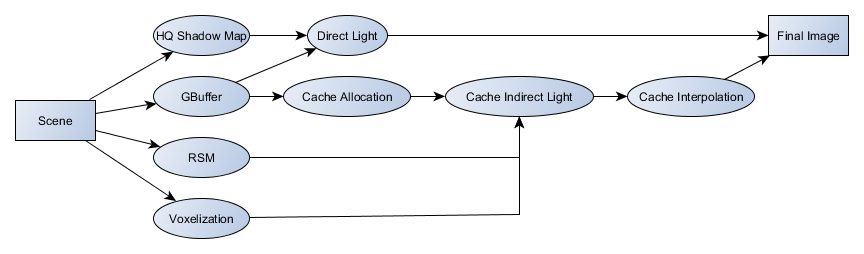
\includegraphics[width=\textwidth]{renderingpipeline_draft}
\end{figure}

\todo{same with image}

\todo{explanation}

\subsection{Cache Allocation} \label{sec:impl:cachealloc}
cacheList via shared memory etc.
"Adress Coord Cache"

\subfilebib % Makes bibliography available when compiling as subfile
\end{document}